\chapter{Quantitative Description Of The Simulation And Reality}
For the evaluation of the effectivity of the containments strategy tested, it is necessary to make the simulation as realistic as possible. Still some assumptions will be made to keep the complexity and runtime reasonable. 
All statistics given here have been provided by Dr. Jörn Gethmann and Dr. Hartmut Lentz \citep{personalCom},\citep{personalCom1} of the FLI for the sake of implementing the simulation. They have been extracted from HI Tier (Herkunftssicherungs- und Informationssystem für Tiere, \citep{HIT}), a nation wide database database containing data about cattle in Germany. All cows need to be registered in this database as soon as they get an ear tag. Every trade needs to be announced here. This means every farmer has to register a cow that left his/her premise and the farmer on the receiving end need to input that he got the cow with the specified ear tag. Every death and every import or export needs to be tracked here as well.
\paragraph{Reliability Of The Data Provided By HI Tier}
According to \citep{personalCom} the data given by HI Tier is very reliable, since it has build in tests for the consistency of the data. For example a farm that did not notify the system that it bought a cow will not be able to tell the system that this cow died. On the other hand it could happen that the wrong ear tag number is put into the system or that farmers do not apply an ear tag before a calf dies, because they want to save money in case the calf dies early. Therefore some errors could occur and the statistics could be wrong.
\section{Breeding Dynamics}\label{chap:breedingDynamics}
The breeding dynamics are the foundation of a working simulation, because they lead to the demography that is necessary for the disease to spread properly, since the development of the disease within the body of a pregnant cow and it's calf is strongly influenced by the time window in which the infection takes place.
The breeding dynamics will be tested on a single farm since trading should have no effect on them\footnote{The single farm is put into a network with a slaughterhouse so that the farm can keep it's size stable by dumping all cows produced.}.
\paragraph{First Calving Time}
The time of the first calving is dependant on multiple distributions:
\begin{itemize}
\item age of first insemination
\item success rate of inseminations
\item rate of aborts
\item duration of pregnancy 
\item time before trying to inseminate a second (or third) time
\end{itemize}
All of these distributions are defined in {\tt Model\_Constants.h} and the distributions put into a random number generator from the gnu scientific library (gsl). All of these distributions have been gathered, but can not directly be observed using the data from HI Tier, which is why we can only compare the results for the first calving time from HIT to the results from our simulation.
The results of the given distributions are shown in plot \ref{fig:firstCalvingTime}. 
It can be seen, that the position of the maximum from the HIT database is met by the results of the simulation quite well. Furthermore the results show that the data in HIT is not completely correct since it contains calvings of cows with an age of $400\,\text{days}$ which is too little since the time of first insemination for most cow races lays between eight and ten months ($240-300\,\text{days}$) and the pregnancy lasts at least nine months ($270\,\text{days}$), making up for a total of at least $510\,\text{days}$. 
\begin{figure}[htbp]
\centering
\noindent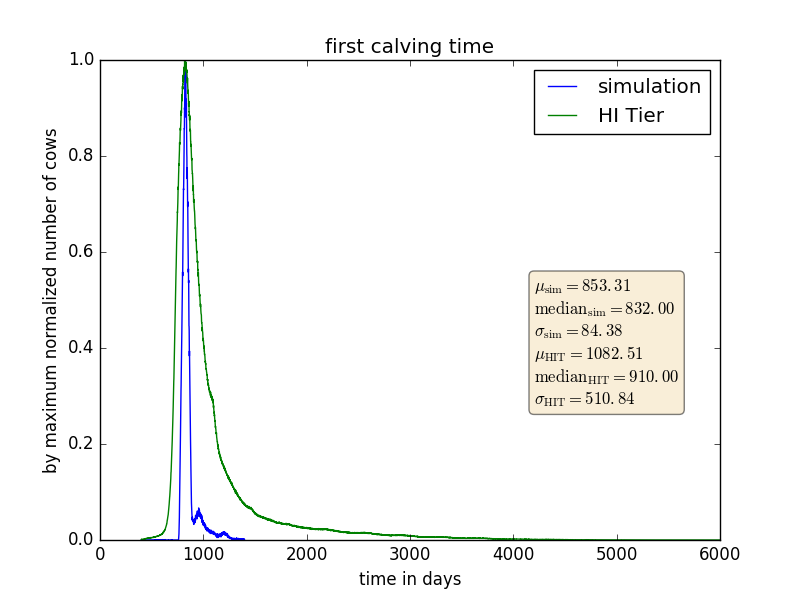
\includegraphics[width=0.8\linewidth,height=\textheight,
keepaspectratio]{firstCalvingTimesNormalwithCSV.png} 
\caption[First Calving Time]{The picture shows the first calving time of all cows in the simulation (blue line) in comparison to the realistic data from HI Tier (green line). Both have been normalized by the maximum number of cows with the given first calving time. The times in the yellow box are given in days.}
\label{fig:firstCalvingTime}
\end{figure}
On the right hand side of the peak the results from the simulation do not match reality all to well. This is mainly due to the fact that the simulation assumes a very simple model for the life cycle of a cow. In reality farmers will make their very individual decisions on when to inseminate their cows based on a lot of factors while the code just assumes that every cow will be inseminated right in the moment when it is possible. For farmers it should not make sense to inseminate a cow after 4 years of living but in reality it does make sense if a small farmer has little money and does not want to replace his cow (,he might even has feelings for). This could lead him to try more often to inseminate the same cow until it finally gets pregnant. 
Even though there is no full explanation for the mismatch on the right hand side of the peak, it can be seen that some features exist in the simulation which also exist in reality. There is a bump seen in the data from the HIT database around a time of $1100\,\text{days}$ which is supposedly caused by abortions. In principle it could also be caused by failed conceptions after an insemination, but the time between inseminations is usually less than a month so it can not account for a delay of roughly $270\,\text{days}$ in comparison to the peak at $827\,\text{days}$. 
A similar bump can be noticed in the data from the simulation. It is shifted a little bit towards smaller values of age, so maybe the time of rest after an abortion is a little bit longer than it was foreseen by the distribution implemented in the code or the highest probability for an abortion is a little bit later. Another feature can be noticed in both: the data from HI Tier as well as the data from the simulation. Again the peak in the simulation data is shifted to the left and even further so than the first peak. This might have the same courses as for the first feature.
All in all it will be assumed that the simulation resembles reality sufficiently accurate. It can be seen that median and expectation value are higher in reality, which would lead to a higher probability for a cow to be infected before being inseminated successfully and therefore to recover and become immune before it finally reaches the state of pregnancy that makes the cow prone to give birth to a PI. The median of the first calving time for the simulation is located at $\text{median}_\text{sim}=853\days $, whereas the median of in reality is located at $\text{median}_\text{HIT}=910\days$. This is about one standard deviation $\sigma_\text{sim} = 84\days$ higher. The difference between the expectation values $\mu_\text{sim}=853\days$ and $\mu_\text{HIT}=1082\days$ is even higher. The most significant difference between the two distributions is the standard deviation. The standard deviation of the data from the HIT database is $\sigma_\text{HTI}=510\days$. It is half the expectation value and shows clearly that the behavior of farmers in reality is not very well defined. Further research could analyze if this would have an impact on the disease dynamics such as the periodicity of outbreaks or the shares of the different compartments in the stable state. 
\paragraph{Intermediate Calving Time}
Just as the time of first calving is dependent on several distributions, the length of the time span between two calvings is also dependent on multiple distributions:
\begin{itemize}
\item time of rest after a calving before the first insemination,
\item probability of a successful insemination after the cow has been inseminated successfully before,
\item rate of an abortion,
\item duration of a pregnancy and
\item time before trying again to inseminate.
\end{itemize}
Picture \ref{fig:intermediateCalvingTime} shows the resulting distribution in the simulation and reality. Again it can be noted that the peaks of both distributions are very close to one another, even though the peak in the simulation is shifted by about $4\,\text{days}$. Compared to figure \ref{fig:firstCalvingTime} the variance in both distributions, but especially the data from the HIT database, is much lower. It shows that the approach of assuming that all farmers behave in the same way is much more realistic for the intermediate calving time then for the time of first calving.
\begin{figure}[htbp]
\centering
\noindent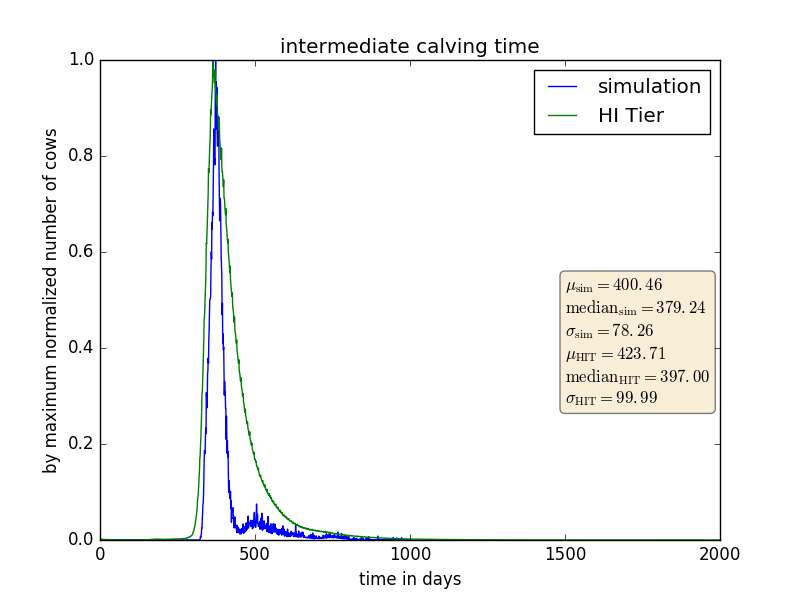
\includegraphics[width=0.8\linewidth,height=\textheight,
keepaspectratio]{intermediateCalvingTimeswithCSV.png} 
\caption[Intermediate Calving Times]{The length of the time between two calvings is shown. Both have been normalized by the maximum number of cows with the given first calving time. The times in the yellow box are given in days.}
\label{fig:intermediateCalvingTime}
\end{figure}
The data from HIT looks similar to a poisson distribution. The distribution's tails of both distributions are close to one another. The second feature of the simulation's data can only be explained by failed inseminations, because the difference between the two peaks is about $130\,\text{days}$, which can not be explained by failed pregnancies. Further side maxima can be observed between five and twenty five days before and after that feature. It is unclear why the slope between the first and second feature in the simulation is much steeper than the observed data from the HIT system. The later median and expectation value can lead to similar results in relation to the the disease dynamics as suggested for the first calving time above, but despite these differences the intermediate calving time is also considered to be sufficiently accurate. Also in this dataset absurd data points like intermediate calving times smaller than duration of pregnancy can be observed, which leads to the same conclusion that the data from HIT seems to contain a lot of wrong entries.\footnote{Werte einfließen lassen}

\section{Disease Dynamics}
To allow for a better understanding of the disease dynamics two simulations with a single farm were have been run. One of them had a herd size of about $400\cows$, while the other had a herd size of $40000\cows$. The latter is quite unrealistic, but still the difference in the herd size can lead to a better understanding of the way how the disease will behave.
\begin{figure}[htbp]
\begin{minipage}{0.5\textwidth}
\centering
\noindent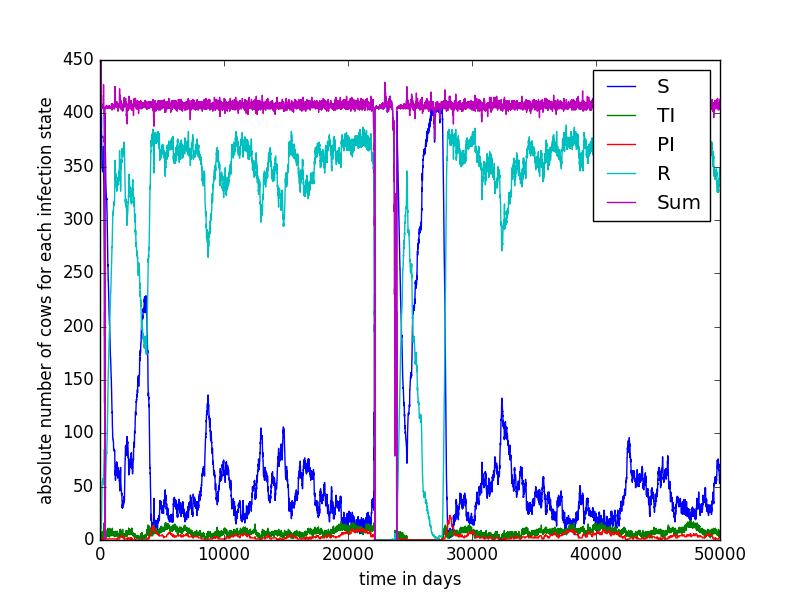
\includegraphics[width=0.9\linewidth,height=\textheight,
keepaspectratio]{totalEndemicNumbers300.png} 
\end{minipage}
\begin{minipage}{0.5\textwidth}
\centering
\noindent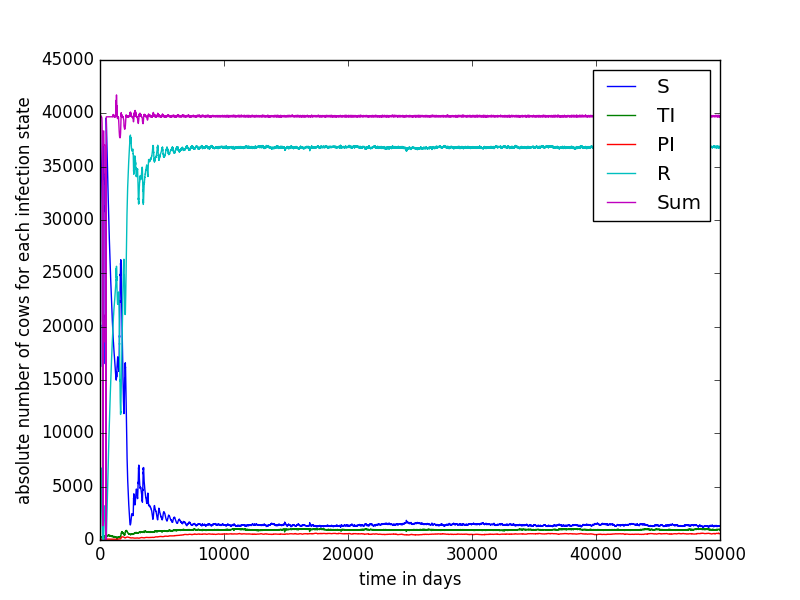
\includegraphics[width=0.9\linewidth,height=\textheight,
keepaspectratio]{totalEndemicNumbers40000.png} 
\end{minipage}
\caption[Absolute Numbers Of Compartments In Different Farm Sizes]{The plots show the absolute numbers of cows of the different compartments: (Susceptible $S$[deep blue], Transiently Infected $TI$[green], Persistenly Infected $PI$[red], Recovered $R$[cyan] and the sum of all of them [purple]). Note that the compartment of recovered contains the animals protected by maternal antibodies too\protect\footnotemark. The left hand graph shows the behavior of a \glqq small\grqq\ farm with roughly $400\cows$ while the graph on the right hand side corresponds to the behaviour of a farm with approximately $40000\cows$.}
\label{fig:absoluteNumbersCompartmentsDifferentFarmSizes}
\end{figure} 
\footnotetext{It would also contain vaccinated animals, but there is no vaccination applied in the simulation which produced these datasets.}

The plots in figure \ref{fig:absoluteNumbersCompartmentsDifferentFarmSizes} illustrate the different behavior of both farms in absolute numbers. Both plots show that the overall farm size is relatively stable. A stable state in terms of the disease spread is reached after less then $10000\days$ in the bigger farm, while the small farm remains relatively unstable. This is also due to the fact that the farm seems to be unable to keep it's size stable. This makes sense because small fluctuations in absolute values still make up for a big change in relative values. Some interesting characteristics shall be commented anyways. Both simulation runs and a number of other test runs have shown the same behavior in the beginning. They have been initialized with a percentage of recovered of $0\,\%$. The number of recovered rises while the number of susceptibles naturally declines. After some time (a few hundred to a few thousand days later) the number of recovered plummets while the number of susceptibles rises again just to fall back to its stable state. This behavior, which resembles the aperiodic boundary case of the a critically damped oscillation, can be found in all simulations. The peculiar behaviour of the smaller farm during which it sells almost all of its cows at some point in time can be found in almost every run with a single small farm. 
The figures \ref{fig:sharesCompartmentsDifferentFarmSizes} show the fractions that the different compartments take up in regards to the total farm size. Both plots show that the distribution for a farm that had contact with a PI given in chapter \ref{chap:rlDataRegulationGermany}  can be met quite well. Since there is no evidence based data on the share of TIs on the whole population \citep{personalCom}, one has to compare the shares of recovereds and PIs. The share of recovered for the bigger farm oscillates around $92\,\%$ and the number of PIs oscillates between $1.3\,\%$ and $1.6\,\%$. The graphs that show the behavior of the smaller farm show a scenario which is more relevant for the simulation as a whole, since farms with a size of $40000\cows$ are not realistic at all. It can be seen that the seropositive population oscillates between $60\,\%$ and $95\,\%$, while the percentage of PIs oscillates between $0\,\%$ and about $6\,\%$. These fluctuations can be explained by the small system size and the resulting relatively big impact of a few animals\footnote{I remember having red a study that said that PIs only made up $40\,\%$ of all infected animals. This would be met by this data, but I couldn't find the study.}. 

\begin{figure}[htbp]
\begin{minipage}{0.5\textwidth}
\centering
\noindent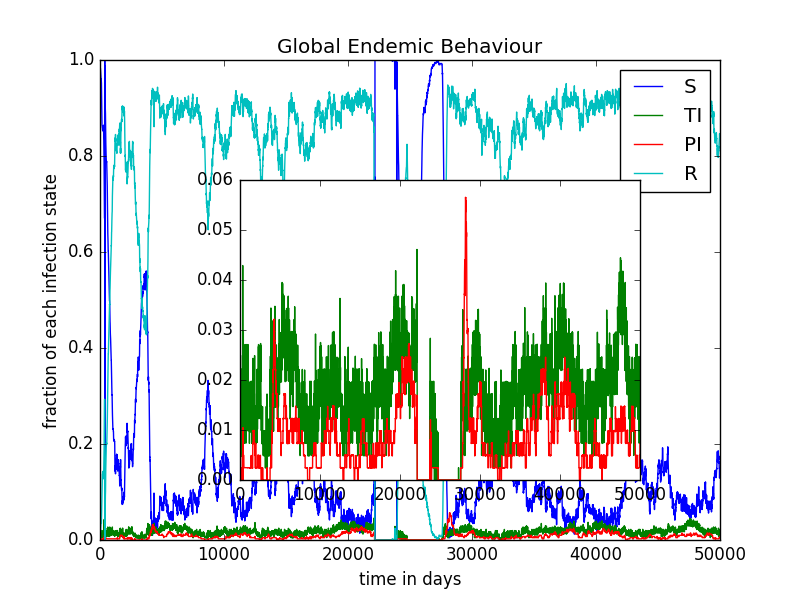
\includegraphics[width=0.9\linewidth,height=\textheight,
keepaspectratio]{endemicFractions300.png} 
\end{minipage}
\begin{minipage}{0.5\textwidth}
\centering
\noindent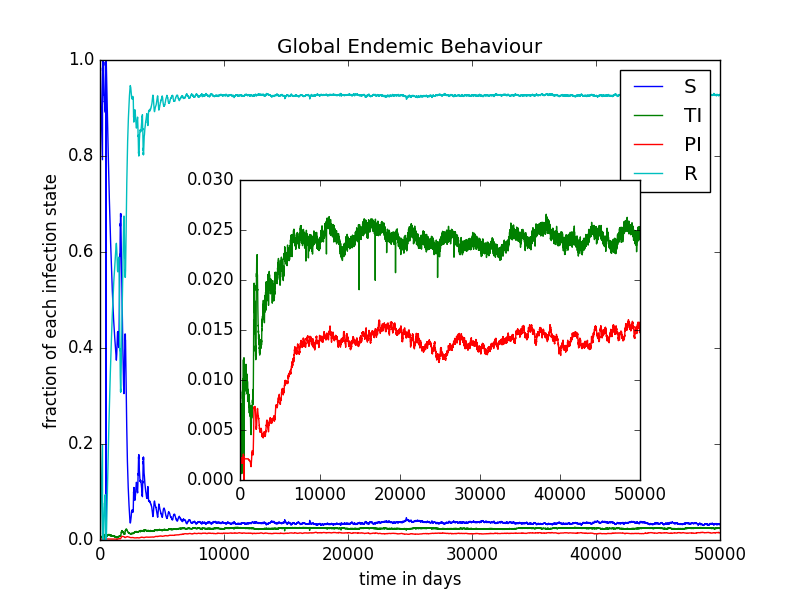
\includegraphics[width=0.9\linewidth,height=\textheight,
keepaspectratio]{endemicFractions40000.png} 
\end{minipage}
\caption[Shares Of Compartments In Different Farm Sizes]{The shown plots display the fractions of the different compartments (Susceptible $S$, Transiently Infected $TI$, Persistenly Infected $PI$ and Recovered $R$) in both examined farms (left: $N\approx 400\cows$, right: $N\approx 40000\cows$). Again the group of recovered individuals $R$ also contains those immune animals which are protected by maternal antibodies.}
\label{fig:sharesCompartmentsDifferentFarmSizes}
\end{figure} 

\section{Trading Dynamics} 
Unfortunately the demography of cattle is not independent from the trading behavior of the different farms which is why they could not be discussed in section \ref{chap:breedingDynamics}. The complex behavior of the market is dependant on a few variables which have been discussed in section \ref{chap:market}:
\begin{itemize}
\item behavior of the cow well farm and slaughterhouse: dump or demand
\item if the market is set to ignore the type of demand a farm announces
\item how farm managers decide which cows to offer
\end{itemize}
At the moment all of these three choices are only binary. This leads to eight different cases which have to be tested. The version which fits reality best will be used to test the different containment strategies. The different scenarios tested in this chapter are shown in table \ref{tab:tradingConfig}.

\begin{table}[htb]
    \begin{center}
    \begin{tabular}{|cccc|}\hline
        \rowcolor{dunkelgrau} \#  & selling strategy & slaughterhouse behavior & ignore type of demand \\\hline
                              1  & oldCowsFirst& dump& true\\\hline
\rowcolor{hellgrau}           2  & oldCowsFirst& dump&  false\\\hline
                              3  & oldCowsFirst& demand& true\\\hline
\rowcolor{hellgrau}           4  & oldCowsFirst& demand& false\\\hline
                              5  & evenlyDistributed&dump& true\\\hline
\rowcolor{hellgrau}           6  & evenlyDistributed& dump& false\\\hline 
                              7 & evenlyDistributed& demand& true\\ \hline
\rowcolor{hellgrau}           8 & evenlyDistributed & demand&  false \\\hline           
\end{tabular}
\caption[Tested Trading Configurations]{This table shows the different trading scenarios tested in this section to resemble reality accurately.}
\label{tab:tradingConfig} 
\end{center}
\end{table}
The other parameters for all of these tests are kept stable. The most important parameters, the rejuvenation rate $\omega$ and the trading interval $dt_\text{trade}$ are chosen as $\omega =27.9\,\%$ (according to \citep{personalCom} and $\text{d}t_\text{trade} = 7\days$. The farm size distribution of Thuringia was chosen for this study with the market implemented as it was described in chapter \ref{chap:market}. In case the slaughterhouse behavior was set to "demand", the number demanded by the slaughterhouse is set to 10000. The simulation is run for a total of $30000\days$

\subsection{Data From HIT}
The plots in figure \ref{fig:demographyGermany} show the time of cattle leaving a farm. Both plots are semi-logarithmic. It can be seen that the graph of the plots roughly follows the trades in shape. This makes sense since all cows need to be traded before they can be slaughtered. For the male cows the peaks in the slaughtered animals make up for $8-10/12$ of the number of trades. In the minimum between the trades make up for $3/12$. The animals which die due to other (natural) reasons make only up for a small percentage of all deaths.


\begin{figure}[htbp]
\begin{minipage}{0.5\textwidth}
\centering
\noindent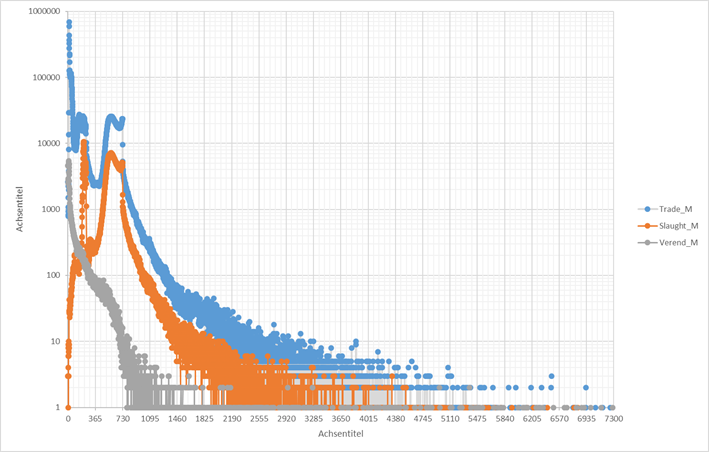
\includegraphics[width=0.9\linewidth,height=\textheight,
keepaspectratio]{Alter_Abgang_M.png} 
\end{minipage}
\begin{minipage}{0.5\textwidth}
\centering
\noindent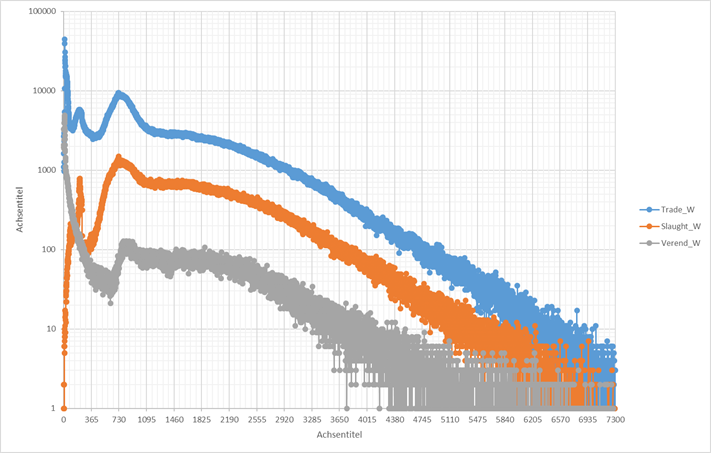
\includegraphics[width=0.9\linewidth,height=\textheight,
keepaspectratio]{Alter_Abgang_W.png} 
\end{minipage}
\caption[Demography Of Cattle In Germany]{The plots show the age of male cows (left) and female cows (right) at the time of leaving the premise in all of Germany. Blue dots mark a cow that left the farm due to a trade, orange dots correspond to cows that where slaughtered and grey dots show a natural death. The plots were generated by \protect\citep{personalCom}. The data is unfortunately not in the possession by the author.}
\label{fig:demographyGermany}
\end{figure} 
For the female cows the slaughtered cows only make up for $10-12\,\%$ of all trades. This could be an indicator that cows are traded multiple times before they are slaughtered. While almost all male cows which die naturally die within the first 2-3 years, female cows seem to be able to live for ten or even twenty years and more. 
This is unexpected because the basic assumption in the setup for the simulation was that cows were going to give births to up 6 calves and then they would be slaughtered anyways. With the given times of first calving and the time between to calvings this would only allow for a lifespan of roughly $3000\days$, including cases of a first calving time of up to $3000\days$ it could explain lifespans of up to $5500$ or even $6000\days$. This again shows that the simple approach that lead to this simulation might be oversimplified. Again a longer lifespan would lead to a higher chance to be recovered, so it might be possible that the number of recovered animals in reality would be higher than the one in the given simulation. 
Note that order of the values in the demography of male cows is one magnitude higher than the order of values in the female plot which could be irritating. Both sexes are born with the same probability, but male cattle are slaughtered earlier. Most cows that were raised to produce meat are sold within the first two years. \citep{steinbach16} found out that roughly a fifth of all farms is made up of fattening farms so it is not surprising to see that male cows in general die much earlier than female cows.
\subsection{Expectations}
One of the scenarios discussed in this chapter is supposed to be used for the studies on the containment strategies. The strategy chosen should have most of the properties of the real data discussed above. Obviously the ages of cows will be less since different statistic used are not matching reality with a hundred percent accuracy. The first calving time alone could lead to a difference of a few thousand days in age between the demography in reality and the simulation. A few things are important: The most important feature is that the trades of female cattle should outnumber the slaughters by about a factor of ten and therefore the following graphs will contain the quotient of both curves as well. Furthermore peaks at about one and two years of age should be clearly visible. The steepness of all three curves should almost be parallel stating at an age of approximately six years. 
In general ignoring the type of the demand should lead to the cows getting older because all cows will get bought all the time and therefore they should stay in the system longer. This should also lead to a number of trades that is much higher than the number of slaughters, since every cow is traded multiple times before it is sent to the slaughterhouse. If the market is set to follow the request of the farms, this will lead to farms only selling pregnant cows. Therefore all other cows will be pushed to the slaughterhouse if it's behavior is set to \glqq dump\grqq. Otherwise these kinds of cows will pile up in the farms because the slaughterhouse might not have the capacity to buy all the leftover cattle on the market.
This means that setting the behavior to dump would in return shorten the lifespan of cows because it is more likely for them to leave the system. 
The selling strategy of the farms could be set to \glqq oldCowsFirst\grqq\ which will make farmers sell worthless cattle, especially bulls first. This should be the best setting to match the male demography of cattle in Germany. When it is set to \glqq evenlyDistributed\grqq, the farm will try to keep it's current demography, so this could have a stabilizing influence on the demography of the system as a whole.
\subsection{Scenario 1}
The plots shown in figure \ref{fig:demographyScen1} exhibit some of the required criteria. The two diagrams will be discussed seperately.
\paragraph{Male Demography}
The demography of male cattle in \ref{fig:demographyScen1}a show that the number of trades is much higher than the number of slaughtered animals throughout all ages, but at least for the first one and a half years it is not bigger by one order of magnitude. For the beginning the number of natural deaths almost follows the fermi-like distribution of reality, but after a year it rises again to a second peak which is not supported by the data presented above, just to rise again before dropping to zero at around $730\days$. 
The rise after approximately $5\,\text{years}$ does not match reality at all. Still the slopes share about the same steepness after around $7\,\text{years}$. The first peak in trades and slaughters appears after about half a year and matches reality quite well, whereas the second peak is not existent at all. Just as in reality most male cows have died after 9 years.
\begin{figure}[htbp]
\begin{minipage}{0.5\textwidth}
\centering
\noindent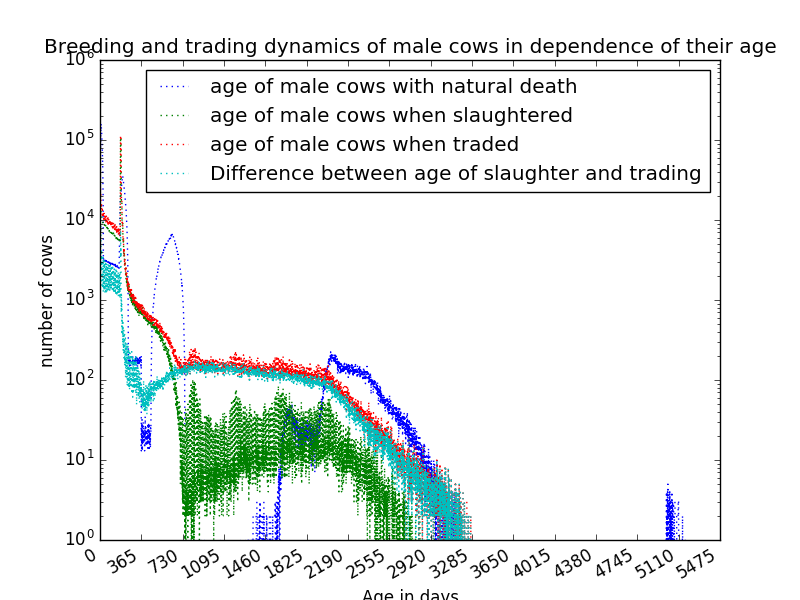
\includegraphics[width=0.9\linewidth,height=\textheight,
keepaspectratio]{scen1maleDemography.png} 
\end{minipage}
\begin{minipage}{0.5\textwidth}
\centering
\noindent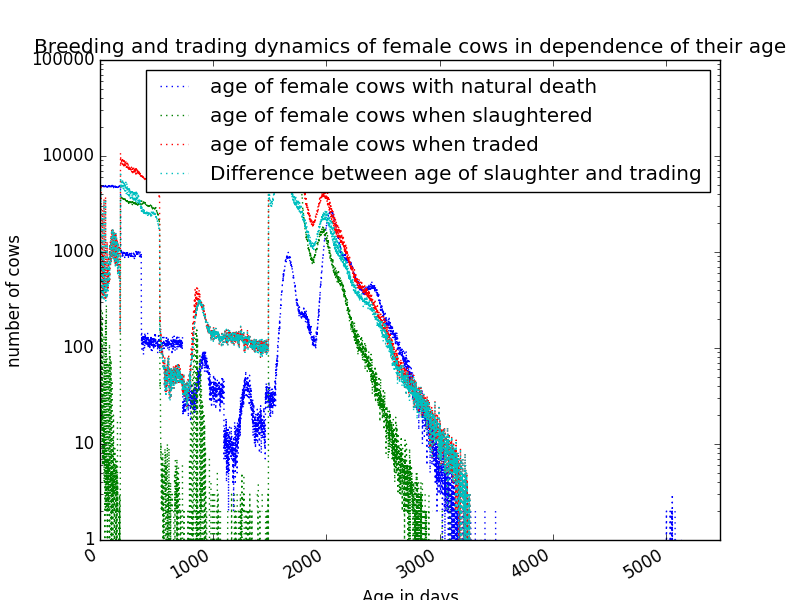
\includegraphics[width=0.9\linewidth,height=\textheight,
keepaspectratio]{scen1femaleDemography.png} 
\end{minipage}
\caption[Demography in Scenario 1]{These plots show the demography of male (left) and female cattle in the first tested trading scenario. The quotient between trades and slaughters is plotted to make it easy to check if there is at least an order of magnitude difference between the two.}
\label{fig:demographyScen1}
\end{figure} 


Maybe this could be improved by setting the natural age distribution differently. If the bulls that die after a year where to be sold, the whole diagram would picture reality surprisingly well.  
\paragraph{Female Demography}
The curves of the female demography have quite similar problems. The number of slaughters is too low for the first four years. After five and a half years all curves have the same steepness. 
A peak at about half a year in trades and slaughters exist which does not diminish until one and a half years, but the second peak at about two years is missing. Another small peak appears at two and half years, but it is not as high as expected: The second peak should be about twice as high in absolute numbers as the fist peak. 
This could be explained by a shift of a big part of animals to a higher age due to the two settings "ignoreTypeOfDemand" and the "selling strategy". Still just as in reality most cows have died after about 9 years which is pretty close to reality.

\subsection{Scenario 2}
This subsection will only focus on the differences of the graph \ref{fig:demographyScen2} of the second scenario towards scenario one which should be inhibited by setting the market to not ignore the type of demand of the different farms which makes them buy pregnant cows only.
\begin{figure}[htbp]
\begin{minipage}{0.5\textwidth}
\centering
\noindent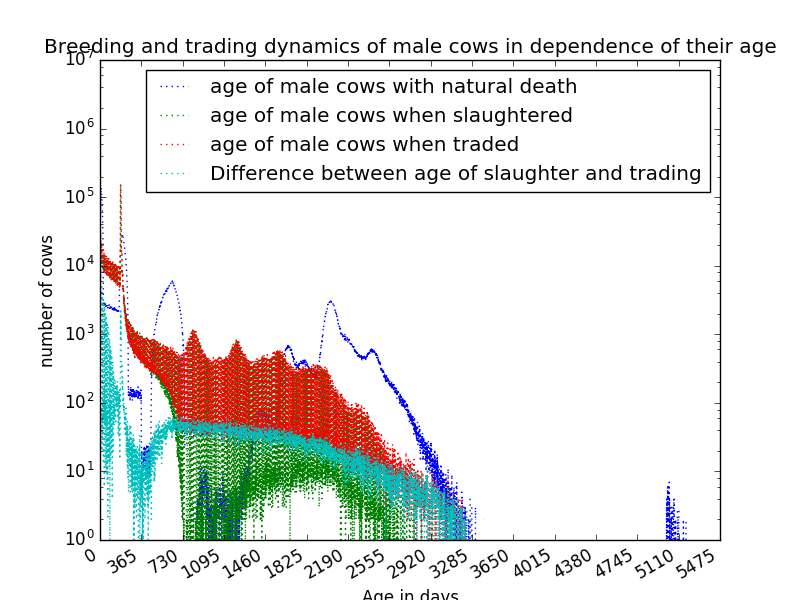
\includegraphics[width=0.9\linewidth,height=\textheight,
keepaspectratio]{scen2maleDemography.png} 
\end{minipage}
\begin{minipage}{0.5\textwidth}
\centering
\noindent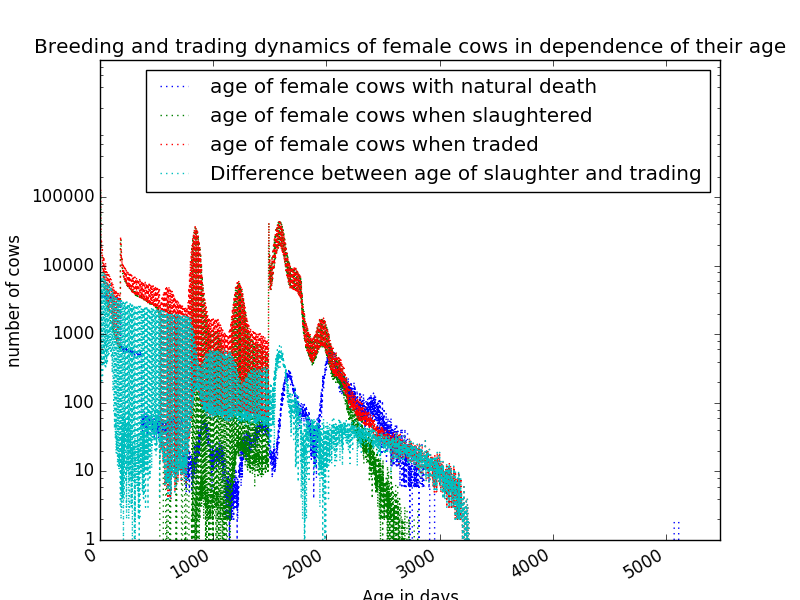
\includegraphics[width=0.9\linewidth,height=\textheight,
keepaspectratio]{scen2femaleDemography.png} 
\end{minipage}
\caption[Demography in Scenario 2]{Plots of the demography of cattle when beeing traded, slaughtered or dying for scenario two of the trading tests.}\label{fig:demographyScen2}
\end{figure} 
\paragraph{Male Demography}
The curve of natural deaths shows pretty much the same trend as it does for scenario one except for the maximum after $2000\days$ which is an order of magnitude higher. This also leads to it being much steeper then in scenario one.
The trading graph also exhibits a behavior pretty close to the one of scenario one for the first year but starts to vary after that. The number of trades seems to oscillate strongly after one year. The minimum of the fluctuations is almost on two thirds of the level of the number of trades in scenario one. The upper end of these fluctuations is about one order of magnitude higher. The maximum age is about one year less than in scenario one. 
The number of slaughters also oscillates just as in scenario one, but the minimum of these fluctuations is much lower, but also the maxima are much higher and seem to be almost as high as the maxima of the number of trades. 

\paragraph{Female Demography}
The graph describing the natural death is again very similar in shape to the graph from scenario one. Most of the numbers are reduced to half of the ones of the first scenario, but the peaks are located at the same positions. The shape is different only in the beginning where it is a little bit less of a step function at the discontinuous points.
The number of trades exposes bigger differences towards the first scenario. It already starts with a number of sold cows twice as high as it was before. The peak afterwards is only a about $20\,\%$ higher than before and declines much faster, rendering the number of trades in the first few year of a female calf almost as high as the first peak at about a year of age. The second peak around years is time actually almost twice as high as the first peak just as it is seen in reality. The only difference towards reality in this early section is that the minimum in between the two maxima should be shifted more towards the first peak whereas it is close to the second peak in this plot. Between the second and third peak of the first plot another feature was created. The shape of the graph looks pretty similar without it, but the new peak is about two thirds as high as the other peaks. The rest of the trading plot is pretty similar to the behavior of the system in the previous scenario. The last peak is again the highest peak of all, which is not in agreement with the reality. 
The number of traded animals is not much higher than the number of slaughtered ones. For the first few years the differences oscillates a lot but after about four years it becomes stable and declines. This is quite intuitive since the farms are not forced to buy any cow so most of the cows offered on the market will be sold straight to the slaughterhouse leading to a far reaching congruency between the number of trades and the number of slaughtered animals. Only in the age between the first pregnancy towards the time of approximately the third calving big oscillations in the number of slaughtered animals can be seen which makes sense, because the farm will try to keep heifers which are ready for breeding, milk cows and pregnant cows as it was discussed in \ref{chap:farmManager}.
\subsection{Scenario 3}
Scenario three will also be compared to the results from the very first scenario mainly, because it only differs in one variable. All cows and requests are put into a single queue, but this time the request of the slaughterhouse for $10000\cows$ per {\tt Cow\_Trade\_Criteria} except PREGNANT will ($9\times 10000\cows = 90000\cows$) be pushed to the demand queue. If one wanted to do a guess of how many cows are sold during the whole run, one could take the maximum of for example the second simulation of about $10^5\cows \times 5500(number of \days) = 5.5\cdot 10^8$ this would give a rather bad estimate of how many cows are sold at maximum! The slaughterhouse could buy $9\cdot 10^4\cows$ every 7\days: 
\begin{equation}
N_\text{bought}^\text{max} = \frac{N_\text{requested}\cows}{\text{d}t[\days]}\times t_\text{tot}[\days] = 9\cdot 10^4 \times \frac{3\days}{7\days}\cdot 10^4 \cows= 3.857...\cdot 10^8\cows.
\end{equation}
This means the slaughterhouse will pretty much buy every cow offered that can not be sold. At the same time it will have to compete with all other farms and the source farm will not be pushed to satisfy all demands at the end of the trading period. This might lead to a shortage of cows. This possibility was falsified summarizing the number of all cows at every step of time. This leaves the expectation, that scenario three should basically behave similar to scenario one, but could be adjusted if the number of cows requested by the slaughterhouse at each trading time was set lower.
\paragraph{Male Demography}
As expected after the explanation above \ref{fig:demographyScen3}a shows an astonihing similarity to \ref{fig:demographyScen1}a. The only real difference is that the number of slaughtered animals stays about the same while the number of trades is about $2-3$ times as high. This makes sense because bulls and male calves are offered with the highest priority. If the farm can not deny buying them because the market ignores the request cow type, male cattle will be tradedvery often before finally reaching the slaughterhouse, which is put at the end of the list of farms and therefore get to request cows at the last position.
\begin{figure}[htbp]
\begin{minipage}{0.5\textwidth}
\centering
\noindent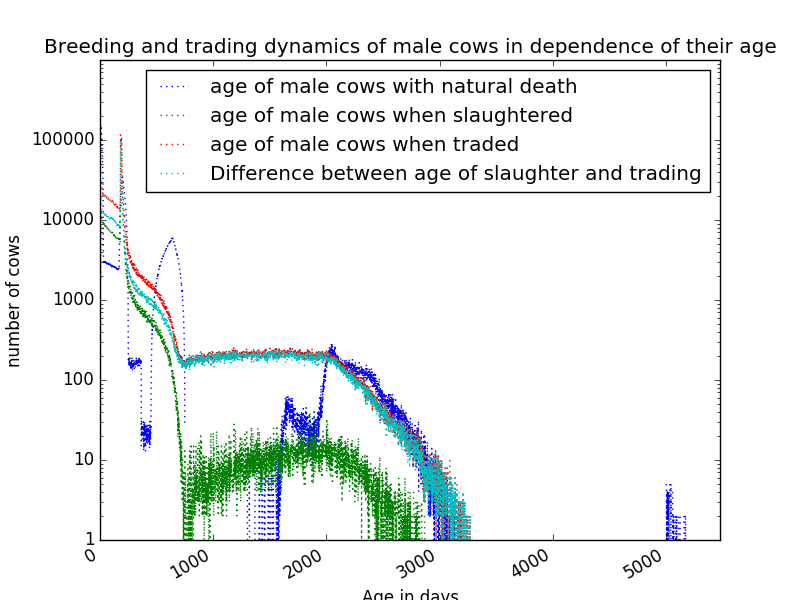
\includegraphics[width=0.9\linewidth,height=\textheight,
keepaspectratio]{scen3maleDemography.png} 
\end{minipage}
\begin{minipage}{0.5\textwidth}
\centering
\noindent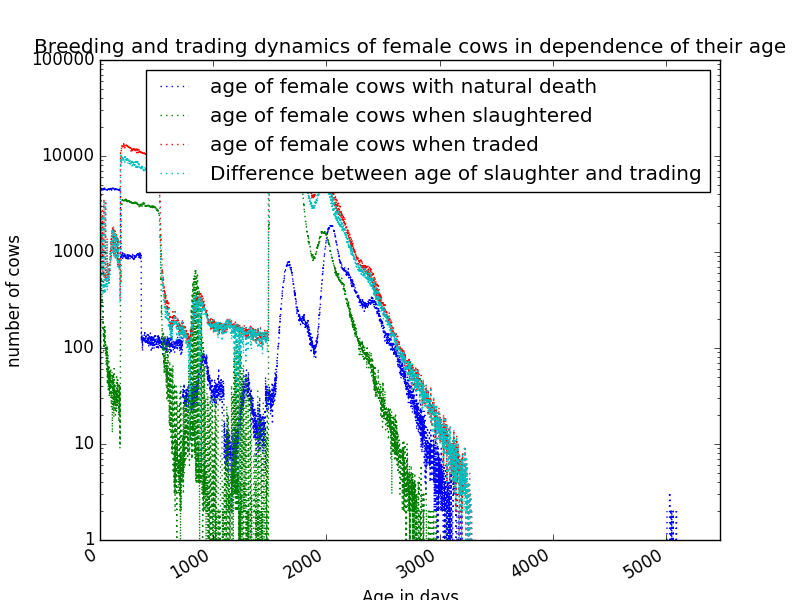
\includegraphics[width=0.9\linewidth,height=\textheight,
keepaspectratio]{scen3femaleDemography.png} 
\end{minipage}
\caption[Demography in Scenario 3]{Plots of the demography of cattle when beeing traded, slaughtered or dying for scenario three of the trading tests.}
\label{fig:demographyScen3}
\end{figure} 
\paragraph{Female Demography}
The female demography shows the exact same behavior as the male demography.

\subsection{Scenario 4}
The graph of this scenario will be compared with the graph of scenario two mostly. Since the kind of demand of farms will not be ignored, only pregnant cows will be bought by the farms. In comparison to scenario three this should lead to all non pregnant cows being sold to the slaughterhouse. In addition to the big number of cows that are requested by the slaughterhouse, this leads to almost all cows being sold to it. The source farm can not supply enough cows to the system. Still a short discussion should take place here.
\paragraph{Male Demography}
The male demography basically just shows the natural death graph. Some male cows get produced, but they get sold right away.
\begin{figure}[htbp]
\begin{minipage}{0.5\textwidth}
\centering
\noindent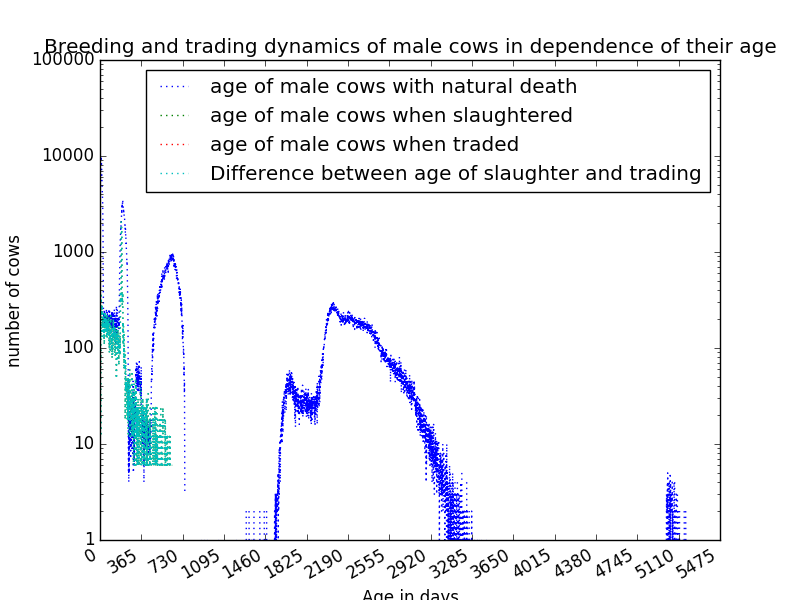
\includegraphics[width=0.9\linewidth,height=\textheight,
keepaspectratio]{scen4maleDemography.png} 
\end{minipage}
\begin{minipage}{0.5\textwidth}
\centering
\noindent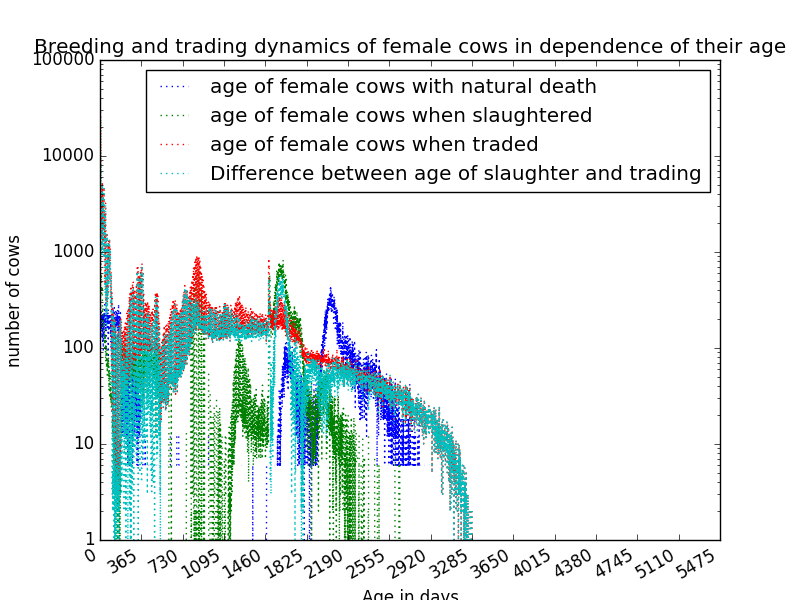
\includegraphics[width=0.9\linewidth,height=\textheight,
keepaspectratio]{scen4femaleDemography.png} 
\end{minipage}
\caption[Demography in Scenario 4]{Plots of the demography of cattle when beeing traded, slaughtered or dying for scenario four of the trading tests.}
\label{fig:demographyScen4}
\end{figure} 
\paragraph{Female Demography}
The female demography resembles the real demography quite well besides the peak around two and a half years. Most likely this peak is due to the cows brought into the system by the source farm. This also explains the big peak in scenario two because more cows are introduced from the source farm.

\subsection{Scenario 5}
Again this scenario will be compared to scenario one because only one variable has been changed in comparison to it. The selling strategy is changed, but farms are still forced to buy all kinds of cows. This will lead to cows being in the system for quite some time. On the other hand farms will try to maintain the demography in male as well as female cows, because they are choosing the number of cows per criteria based on their share on the total population. This should lead to a less steep curve in both male and female cows and less peaks.
\paragraph{Male Demography}
The number of trades is pretty much the same as in scenario one, but the number of slaughters oscillates much stronger. Other than that not much of a difference can be seen.
\begin{figure}[htbp]
\begin{minipage}{0.5\textwidth}
\centering
\noindent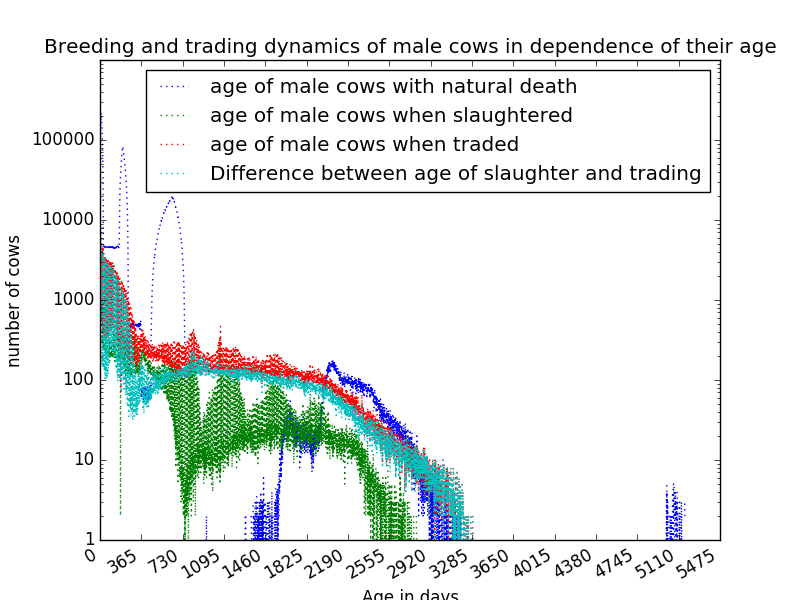
\includegraphics[width=0.9\linewidth,height=\textheight,
keepaspectratio]{scen5maleDemography.png} 
\end{minipage}
\begin{minipage}{0.5\textwidth}
\centering
\noindent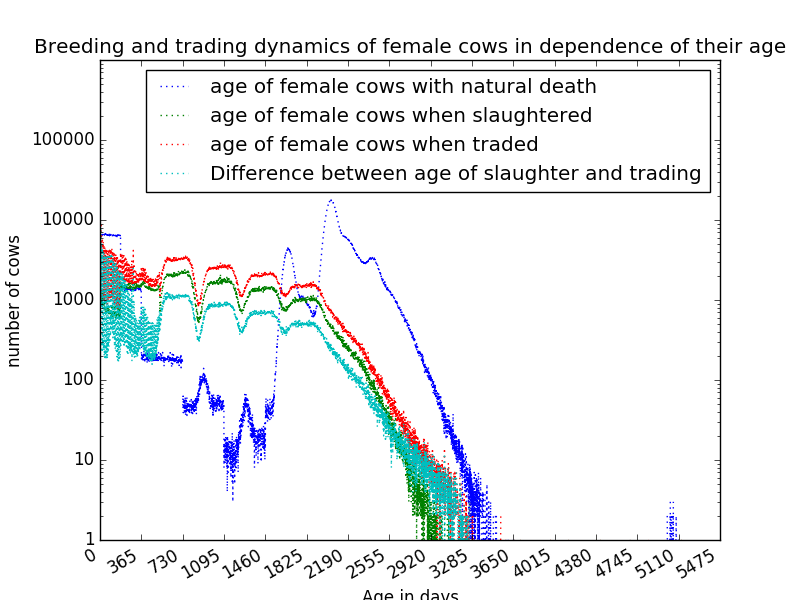
\includegraphics[width=0.9\linewidth,height=\textheight,
keepaspectratio]{scen5femaleDemography.png} 
\end{minipage}
\caption[Demography in Scenario 5]{Plots of the demography of cattle when beeing traded, slaughtered or dying for scenario five of the trading tests.}
\label{fig:demographyScen5}
\end{figure} 
\paragraph{Female Demography}
The graph shows a much lower but also more steady curve of trades that is interrupted multiple times about once a year for about two hundred days.


\subsection{Scenario 6}
Scenario six can be compared to scenario two and five. In comparison to scenario two the trading curves should be more steady. In comparison to scenario five the number of slaughters could oscillate as much as the number of slaughters in scenario two is oscillating in comparison to scenario one.
\paragraph{Male Demography}
The number of trades oscillates far more than the number of trades and the number of slaughters oscillate more than in scenario five, but less then in scenario two. The overall number of trades is much lower then in scenario two and a little bit steeper then in scenario five. 
\begin{figure}[htbp]
\begin{minipage}{0.5\textwidth}
\centering
\noindent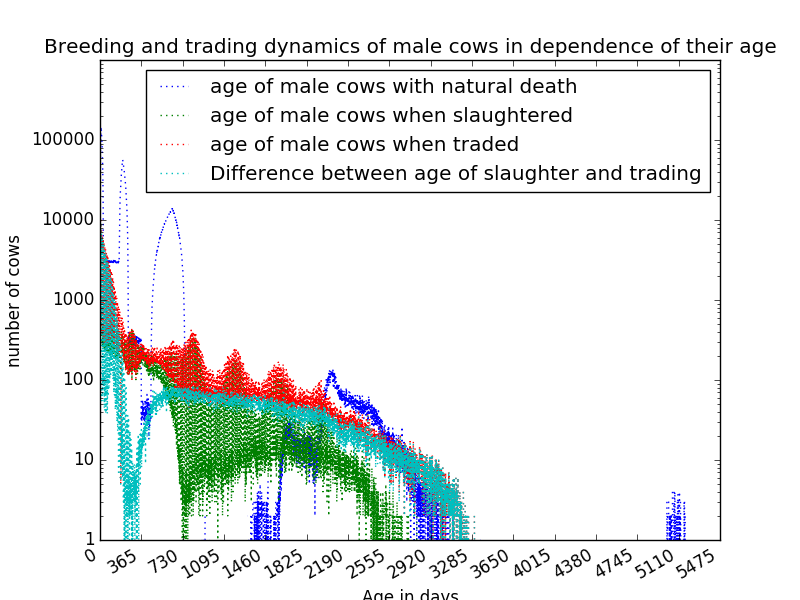
\includegraphics[width=0.9\linewidth,height=\textheight,
keepaspectratio]{scen6maleDemography.png} 
\end{minipage}
\begin{minipage}{0.5\textwidth}
\centering
\noindent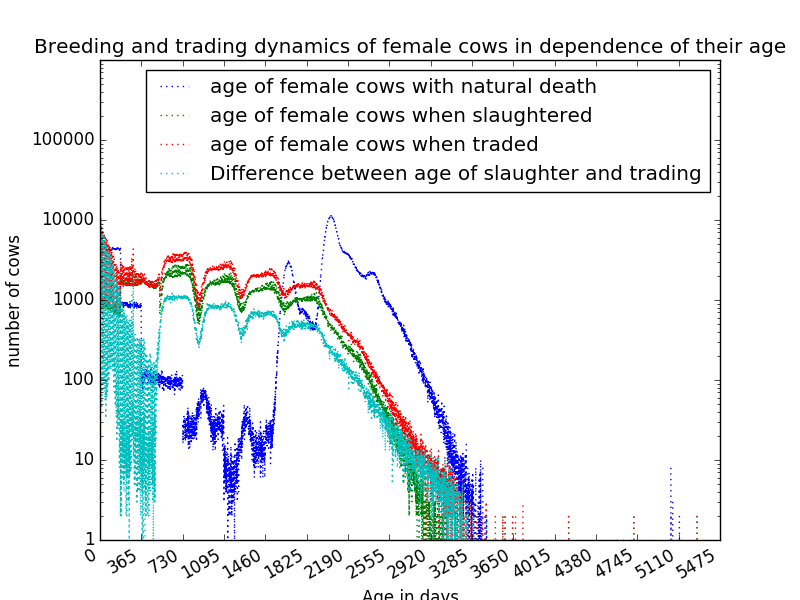
\includegraphics[width=0.9\linewidth,height=\textheight,
keepaspectratio]{scen6femaleDemography.png} 
\end{minipage}
\caption[Demography in Scenario 6]{Plots of the demography of cattle when beeing traded, slaughtered or dying for scenario six of the trading tests.}
\label{fig:demographyScen6}
\end{figure} 
\paragraph{Female Demography}
The number of trades is a little bit higher than in scenario five, but other than that there is not much of a difference to be seen.
\subsection{Scenario 7}
Scenario seven will be compared to scenario three and five. It has been tested again if the number of cows in the system diminishes, but it does not.
\paragraph{Male Demography}
Again it can be seen that the curve over all is much more steady in comparison to scenario three. The first peak at around half a year is almost completely missing. It can also be seen that way less trades take place for cows of age less than two years. After that the curves almost look the same. The higher number of trades in scenario three is also inducing a way higher number of slaughters.
In comparison to scenario five the use of the different slaughter house behavior mainly induces a lesser number of trades for the first two years too. On the other hand one can see features around halve a year and one year. Another noticeable difference is the fact that the numbers of trades and slaughters are oscillating far less. After the age of two years more bulls get traded than in scenario five. 
\begin{figure}[htbp] 
\begin{minipage}{0.5\textwidth}
\centering
\noindent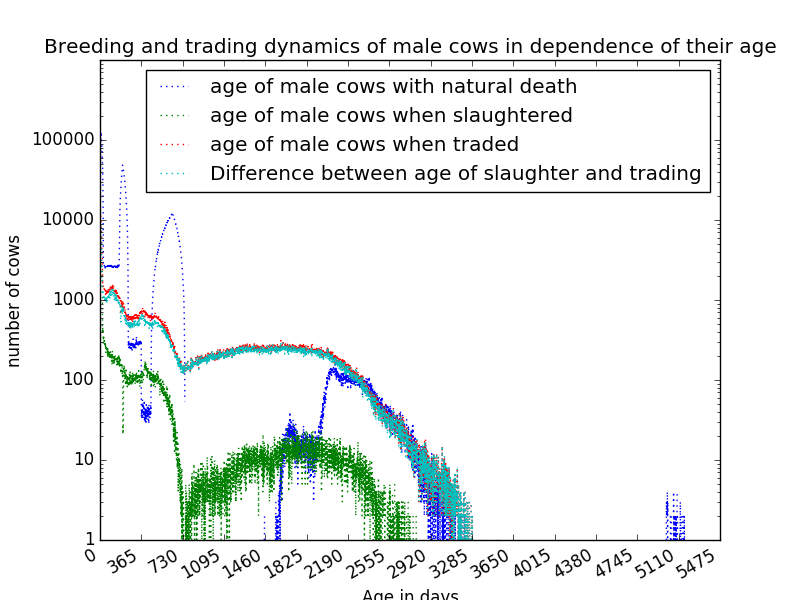
\includegraphics[width=0.9\linewidth,height=\textheight,
keepaspectratio]{scen7maleDemography.png} 
\end{minipage}
\begin{minipage}{0.5\textwidth}
\centering
\noindent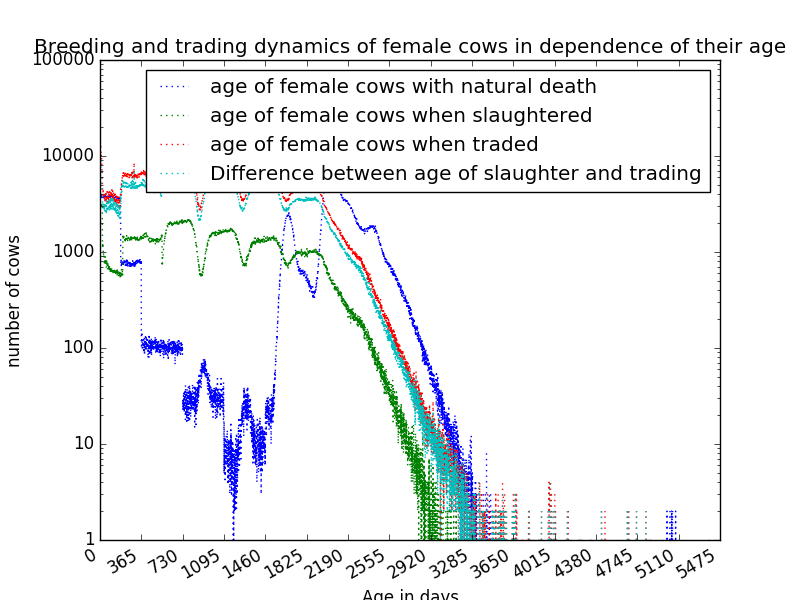
\includegraphics[width=0.9\linewidth,height=\textheight,
keepaspectratio]{scen7femaleDemography.png} 
\end{minipage}
\caption[Demography in Scenario 7]{Plots of the demography of cattle when beeing traded, slaughtered or dying for scenario seven of the trading tests.}
\label{fig:demographyScen7}
\end{figure} 
\paragraph{Female Demography}
In comparison to scenario three the number of trades for the lower in the beginning and the number of trades is in general for steady. The number of slaughters follows the number of trades relatively closely. The steepness of trades and slaughters is about the same in the end as the steepness of the natural deaths. The most interesting thing to mention is that there are in fact trades and slaughters between the ages of nine and fifteen years, which has no precedence in the other scenarios.
In comparison to scenario five the only difference is that the numbers of trades and slaughters and therefore also the difference of the two is oscillating far more.



\subsection{Scenario 8}
Scenario eight could be compared with scenarios four, six and seven. It has been tested if more or less all cows are sold to the slaughterhouse, but they are not. The total number of cows declines durign the first $9000\days$, but it recovers to it's original size after that.
\paragraph{Male Demography}
The male demography again shows mainly the natural death curve of male cows. 
\begin{figure}[htbp]
\begin{minipage}{0.5\textwidth}
\centering
\noindent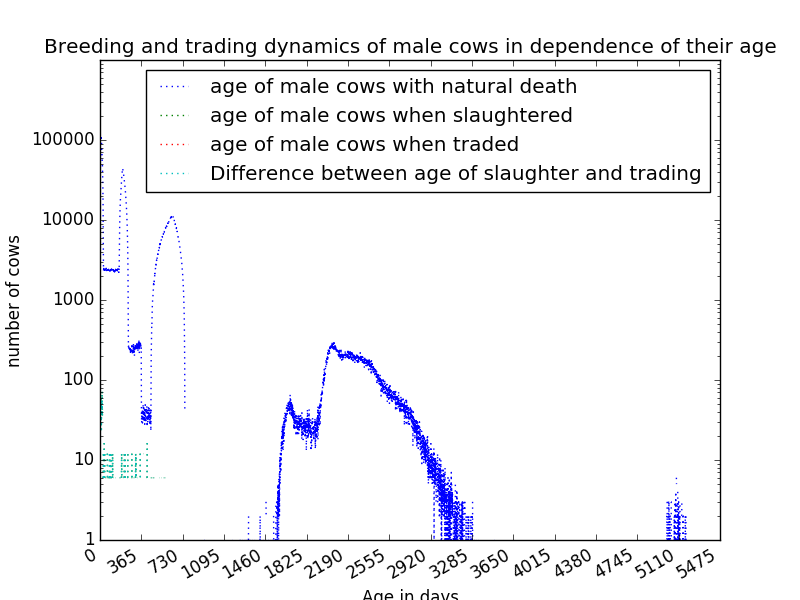
\includegraphics[width=0.9\linewidth,height=\textheight,
keepaspectratio]{scen8maleDemography.png} 
\end{minipage}
\begin{minipage}{0.5\textwidth}
\centering
\noindent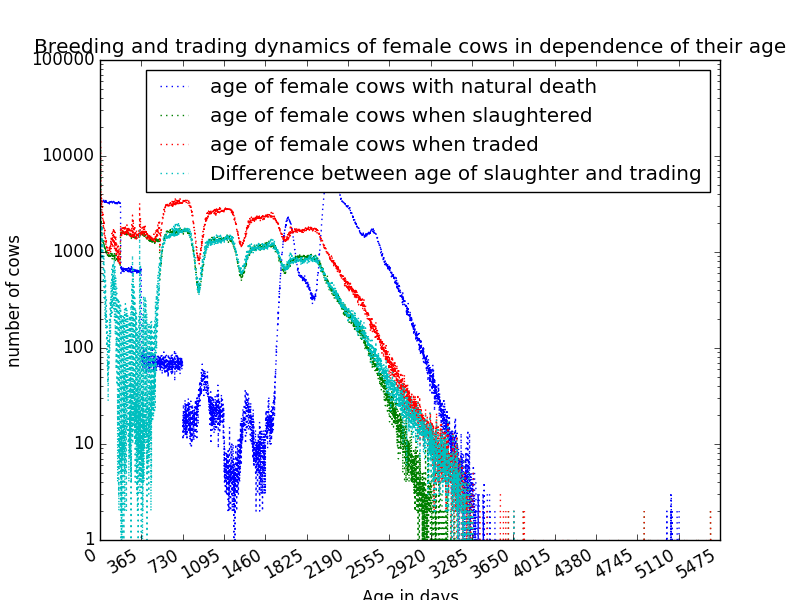
\includegraphics[width=0.9\linewidth,height=\textheight,
keepaspectratio]{scen8femaleDemography.png} 
\end{minipage}
\caption[Demography in Scenario 8]{Plots of the demography of cattle when beeing traded, slaughtered or dying for scenario eight of the trading tests.}
\label{fig:demographyScen8}
\end{figure} 
\paragraph{Female Demography}
The number of trades is much less then the number of trades for scenario seven. Compared with scenario six the number of slaughters is much less. The number of slaughters is exactly half the number of trades for all ages. 

\subsection{Conclusion}
The results presented require a very detailed discussion. From the perspective of optimizing the demography of the system as a whole for male cattle the reason for naturals deaths for them require a big change. If the naturals deaths within the second year of their lives would contribute to trades rather than natural deaths, the curves from scenarios one to three would match the ones from reality much better.
In general the number of trades and the number of slaughters should be much higher than the number of natural deaths. The number of trades is way to low for all of the scenarios given above. This could be changed by either influencing the number of trades or the existence of DEATH-Events, which are currently shown as natural deaths in the graphs, because according to the graphs provided for the demography of cows traded in reality show clearly that the numbers of trades and slaughters should be much higher than the number of natural deaths. 
For now only the female demography will be considered, because it is much more influential for the spreading of disease since only female cows can give birth to new PIs. Therefore all Scenarios but scenario four and eight should provide a demography of male cattle that should be sufficient for any further tests. Scenarios one to three provide high numbers of trades which are most of the time much higher than the number of natural deaths, but expose big peaks which are more flattened in scenarios five to seven. Only scenario two exposes a much bigger number of trades, but it shows a peak that represents the cows introduced by the source farm. The effects of that can not easily predicted, but most likely it makes the results of the whole simulation less realistic. 
Of the scenarios five to seven seven exposes the most trades overall, number of trades that is much higher than the number of slaughters and most of the time it is also higher than the number of natural deaths. Furthermore it has the same steepness in the end of the plot in all three curves and exposes trades, slaughters and natural deaths after the age of nine years. It seem to be the most realistic demography produced within the tested scenarios. The corresponding male demography looks quite reasonable too. It misses the two preaks in the numbers of trades and slaughters at low ages, but since the naturals deaths are still taking place at these ages, the male calves will still be removed out of the system. For all of these reasons, the settings of scenario seven will be used for all further simulations. Another advantage of this is that the selling strategy "evenly distributed" will also try to maintain the demography of the herd leading to little to no male cows being left in the herd after every trading step.
\section{Transients}
The system exposes an oscillating behavior. If the state at the point of initialization is not set to it's stable position, it needs some time to reach this state. This chapter tries to give some insights on these transients.
\subsection{Trades}
Figure \ref{fig:tradingTransients} shows the trading activity of the whole system. It can be seen that absolute numbers of the enveloping functions of all three curves a falling exponentially within the first ten thousand days. Furthermore it can be seen that the number of farms selling cows is much higher than the number of farms buying any. 
\begin{figure}[htbp]
\centering
\noindent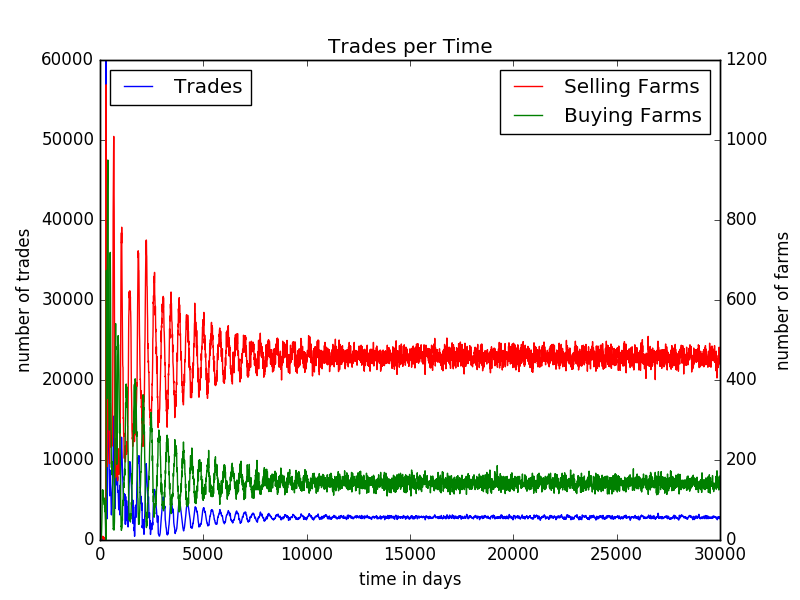
\includegraphics[width=0.8\linewidth,height=\textheight,
keepaspectratio]{scen7tradingPlot.png} 
\caption[Transients In Trading]{The plot shows the number of trades over time. It shows that the system takes some time to get to a point where this number is relatively stable.}
\label{fig:tradingTransients}
\end{figure}


\subsection{Endemic Behavior}
Figure \ref{fig:endemicTransients} shows the endemic development of the system following trade scenario seven. It can be seen that the total number of all cows in the system as well as the fractions of the different compartments are oscillating quite strongly in the beginning. After about seven thousand days only few oscillations are visible, after ten thousand days almost none are to be seen.
\begin{figure}[htbp]
\begin{minipage}{0.5\textwidth}
\centering
\noindent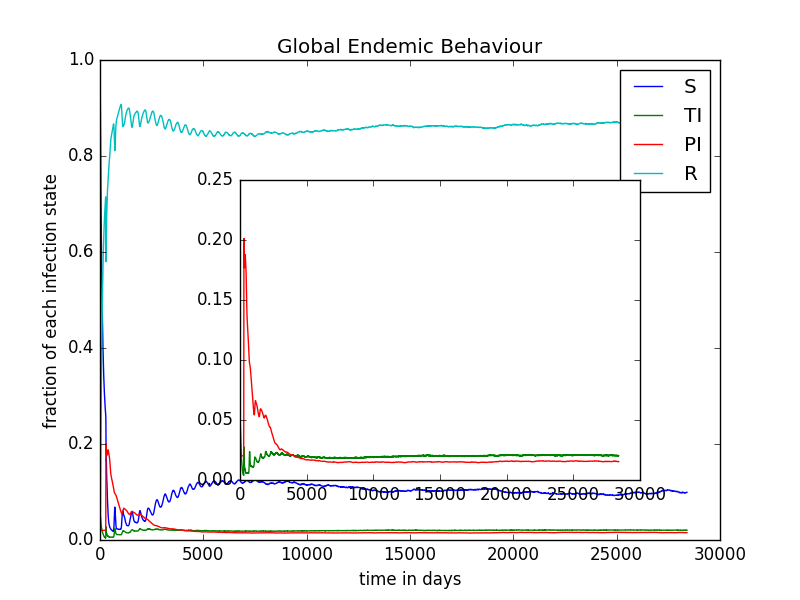
\includegraphics[width=0.9\linewidth,height=\textheight,
keepaspectratio]{scen7endemicFractions.png} 
\end{minipage}
\begin{minipage}{0.5\textwidth}
\centering
\noindent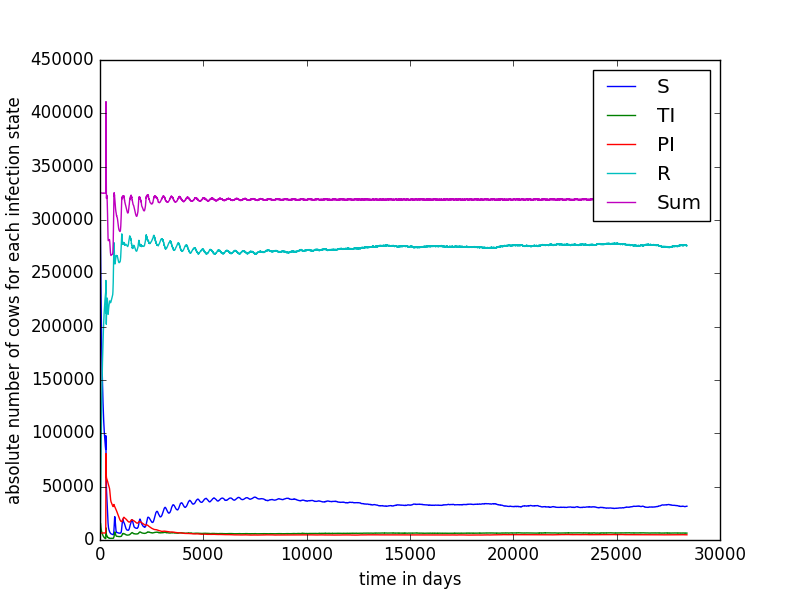
\includegraphics[width=0.9\linewidth,height=\textheight,
keepaspectratio]{scen7totalEndemicNumbers.png} 
\end{minipage}
\caption[Endemic Transients]{}
\label{fig:endemicTransients}
\end{figure} 


\subsection{Conclusion}
For the different tests of the containment strategies the transients will be cut off and neglected. To ensure that the starting conditions are the same, the seed for all simulations will be set the same so that the first ten thousand days will be the same.